\chapter{Requirements Engineering Research}

\section{Overview}

On completion of the initial provenance replay software, we began a requirements
engineering process consisting of requirements elicitation by focus group, and
requirements validation using Technology Acceptance Model (TAM) \parencite{davis_perceived_1989}
and Net Promoter Score \parencite{reichheld_one_2003} (NPS)-based survey
instruments. Approval for NAU IRB project 1804166-3 was received for this study,
including for the recording and transcription of focus group participant
conversations.

Recruitment was conducted through posts on the QIIME 2 forum and through direct
communication with members of the QIIME 2 community. Twenty-five individuals
expressed interest. Twenty-four of these completed the informed consent.
Twenty-three of these were responsive after consent. Four one-hour software
demonstration/focus group sessions were scheduled using the Zoom video
conferencing platform. Once scheduled, each participant was sent a formal
invitation with a link to the zoom meeting, and a reminder email 15 minutes
prior to that meeting with the zoom link. Twenty-three participants were
scheduled. One of these participants canceled prior to participation. One of
these participants left the demonstration prior to the beginning of the focus
group, and the other 21 stayed for the duration. All participants were asked to
complete the survey by email immediately after the focus group. All participants
were sent one survey reminder email within one week of their session. Nineteen
individuals completed the followup survey, taking approximately seven minutes to
do so on average (mean: 7:18, median: 6:07).

Each one-hour focus group session began with a demonstration of the Provenance
Replay software lasting roughly 25 minutes, followed by a discussion of 4-7
questions about the software intended to elicit open-ended feedback and
exploration of possible features of value. Focus group sessions were not always
of adequate length to accommodate all questions from the script, in which case I
tried to select the most impactful questions for requirements elicitation. The
focus group script can be found in Appendix \ref{app:FGScript}.

The survey implement (Appendix \ref{app:survey}) consists of:
\begin{itemize}
    \item background questions we can use to better understand users’ experience
        and attitude relative to QIIME 2, provenance tracking, and computing tasks
    \item eight Likert questions targeting TAM Perceived Ease of Use (PEOU)
    \item twelve Likert questions targeting TAM Perceived Usefulness (PU)
    \item one Net Promoter Score (NPS) question
    \item one select-many question - which demonstrated features you will use?
    \item one ranking question - rank demonstrated features from most to least valuable
\end{itemize}

\section{Results}

\subsection{Net Promoter Score Results}

When asked how likely they were to recommend Provenance Replay features to a
friend or colleague who uses QIIME 2, 78.95\% of participants (15/19) were
classified as promoters (scores of 9-10 out of 10), 21.05\% (4/15) as passive
(scores 7-8 out of 10), and none as detractors, resulting in a net promoter
score of +78.95\%, which is generally considered to be very good. (Figure \ref{fig:NPS})

\begin{figure}[htbp]
\centering
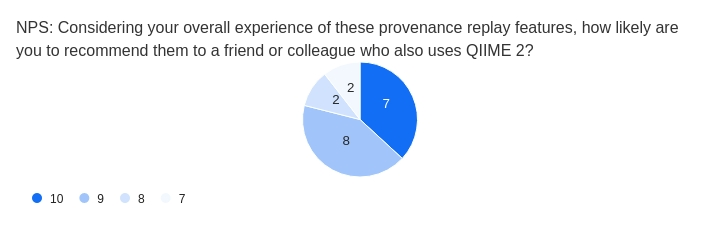
\includegraphics[width=\textwidth]{figures/NPS.jpg}
\caption[Pie chart of net promoter score responses]%
{Pie chart of net promoter score responses, showing seven responses at the
highest value (10), eight at the second highest (9), and two responses each at 8
and 7. No responses rated below 7.}
\label{fig:NPS}
\end{figure}

Though there is still considerable academic debate about the value and
limitations of NPS as a predictive measure \parencite[Table 1]{baehre_use_2022},
it is widely used and less frequently criticized as a measure of “how we are
doing right now”. Our high NPS seems to indicate that users believe this
software is currently worth recommending to others.

\subsection{Technology Acceptance Model (TAM) Results}

Provenance Replay also scored well on the Technology Acceptance Model
instruments. All PEOU questions were framed to ensure that increased ease of use
correlates with a higher numerical score (scaled from 1-7). We assume that all
response sentiment options are evenly distributed across the scale. Similarly,
all PU questions were framed to associate higher perceived usefulness with a
higher numerical score. (Table \ref{tab:scaled_likert_vals})

\begin{table}[htp]
        \begin{tabular}{|p{0.08\textwidth}|p{0.08\textwidth}|p{0.08\textwidth}|p{0.3\textwidth}|p{0.3\textwidth}|}
        \hline
        Score & From  & To    & Response          & Verbal Interpretation \\ \hline
        1     & 1     & 1.857 & Strongly Disagree & Very low              \\
        2     & 1.857 & 2.714 & Disagree          & Low                   \\
        3     & 2.714 & 3.571 & Somewhat Disagree & Somewhat Low          \\
        4     & 3.571 & 4.429 & Neither           & Neither               \\
        5     & 4.429 & 5.286 & Somewhat Agree    & Somewhat High         \\
        6     & 5.286 & 6.143 & Agree             & High                  \\
        7     & 6.143 & 7     & Strongly Agree    & Very high             \\ \hline
        \end{tabular}
    \caption[Scaled likert values for TAM interpretation]%
    {Scaled likert values evenly distribute the ranges to which we map our mean values}
    \label{tab:scaled_likert_vals}
\end{table}

All questions received mean scores of 5.36 or greater, indicating at least a
“high” PU or PEOU for all questions. One question had a median score of 5,
(“slightly agrees”) three had a median score of 7 (“strongly agrees”), and
the rest scored a median of 6 (“agrees”). Respondents rated Perceived Ease of
Use as “high”, with an overall mean of 5.82. Respondents rated Perceived
Usefulness as “high”, with an overall mean of 5.96.

Both PEOU and PU survey sections ended with “overall success” questions.
Respondents “strongly agree” that “Overall, [they] believe these features are
easy to use,” (mean 6.21, median 6) and “strongly agree” that “These features
are useful for me as a QIIME 2 user” (mean 6.16, median 7). With high PEOU and
POU, respondents indicate a positive general attitude toward using Provenance
Replay. Complete TAM results are available in Appendix \ref{app:TAM}

\subsection{Participant Technology Use and Attitude}

According to the TAM, external variables are contributing factors in PEOU and
PU. We gathered information about respondent technology use and attitude, as
these seem likely to influence perceptions and by extension likelihood of
technology uptake.

Respondents had very high rates of command shell use (mean 6.53, median 7), high
average comfort using programming languages (mean, 5.79, median 7, variance
relatively high at 2.38), high average comfort using QIIME 2 (mean 5.84, median
6), and somewhat high average comfort using QIIME 2’s provenance tracking
features (mean 4.68, median 5). Participants were somewhat satisfied with their
current QIIME 2 analysis workflow (mean 4.74, median 5.00), and somewhat agreed
that QIIME 2’s existing provenance tracking features are a useful tool in their
current analysis workflow (mean 4.95, median 5.00).

Respondents reported a very high level of enjoyment in learning to use new
computational tools (mean 6.53, median 7), and somewhat agreed that it is
generally easy for them to learn to use them (mean 5.21, median 5). They agreed
that they “enjoy using QIIME 2” (mean 5.95, median 6), and agreed that it is
generally easy for them to learn new things in QIIME 2. 

Overall, our cohort self-reports as highly computationally inclined, with
attitudes and beliefs about themselves that seem likely to encourage the
adoption of new technologies. This should be taken into account when considering
the strong NPS and TAM results. Complete results available in Appendix \ref{app:techUse}.

\subsection{Feature Use and Rankings}

When asked to select all features they expected to incorporate into their
analyses:

\begin{itemize}
    \item 84\% of respondents believed they would use provenance replay to
        generate citations from their analyses
    \item 84\% of respondents believed they would generate new replay scripts from analysis results
    \item 74\% of respondents believed they would use QIIME 2’s existing
        provenance tracking features (including q2view provenance graphs)
    \item 32\% of respondents believed they would use Checksum Validation
\end{itemize}

These results are promising, indicating that a significant majority of
respondents believe the core replay tools implemented here will become part of
their QIIME 2 workflow.

A second question asked respondents to rank these four features in order of
value, where one represents the most valuable and four represents the least
valuable. Checksum Validation was \textit{by far} perceived as the least valuable feature
to our respondents (mean 3.67, median 4.00), while the three other features
clustered around 2, indicating a relatively even distribution of preference
between these three features, with provenance replay rating slightly higher than
the others, and citation replay slightly lower. (Table \ref{tab:feature_rankings})


\begin{table}[htp]
    \centering
    \begin{tabular}{|p{0.3\textwidth}|p{0.1\textwidth}|p{0.1\textwidth}|p{0.1\textwidth}|}
    \hline
    Feature             & Mean & Median & SD  \\ \hline
    Provenance Replay   & 1.83 & 1.5    & .96 \\
    Provenance Tracking & 2.11 & 2      & .94 \\
    Citation Replay     & 2.39 & 2      & .89 \\ \hline
    \end{tabular}
    \caption[Respondent rankings of feature value]%
    {Rankings of feature value were tightly clustered around the center for the
    three better-performing features. Checksum validation, not included here,
    was clearly the least valued feature. Complete results are available in
    Appendix \ref{app:featureUse}.}
    \label{tab:feature_rankings}
\end{table}

\subsection{Potential confounders}

Confounding effects may exist. Many study participants were recruited from
research groups with professional associations with our laboratory group. The
popularity of the QIIME 2 Platform might convey an inflated sense of value. The
moderator’s role as developer may complicate participants’ ability to share
negative feedback. Participants might believe that by participating in the
demonstration they have received early access to tools that might benefit their
work. In all of these, agreeableness or perceived authority could drive
acquiescence bias, inflating our TAM scores and contributing to our very high
NPS.

Provenance Replay is available to users free of charge. The impact of cost on
PEOU is beyond the scope of this study, but could be an interesting topic for
further research. I have been unable to identify academic publications
benchmarking NPS when applied to Free and Open Source Software (FOSS) like QIIME
2 and Provenance Replay, but it seems reasonable to believe that free products
might also be more likely to receive higher than average NPS or TAM scores.

Finally, these scores are all based on a prepared demonstration of a product
pre-installed in a working computing environment. Though I have made best
efforts to package and document the software to make installation and use
straightforward, all survey metrics, and Perceived Ease of Use especially, could
shift dramatically if users have a different experience working with the
software independently than they did while it was demonstrated by its developer.
Time and recruitment constraints made hands-on sessions unfeasible, but further
work would benefit from reporting based on active software use.


\section{Focus Groups and feature elicitation}

Our primary goal in conducting focus groups was to provide open enough lines of
communication for people to freely share experiences, preferences, and ideas for
how Provenance Replay can be improved or extended to meet their needs most
effectively. Deriving meaning from loosely structured conversations is subject
to significant interpretive bias, but I have done my best to value different
types of feedback equally. Each recording was reviewed in full, and any
statements that I felt were relevant to the current usage of QIIME 2’s
provenance capture tools, the demonstrated state of Provenance Replay, or
potential future development of Provenance replay were noted. 

These notes took two primary forms, often used in parallel. In the first, I
attempted to capture the core intent of the statement in paraphrase, recording
the paraphrased statement if it was novel, or incrementing a counter next to an
appropriate existing paraphrase if one existed. For example, three people
expressed that they “like the citation feature.” I recorded the paraphrase with
a 1 counter when I first encountered the sentiment, and simply incremented the
counter on the second and third occurrences. This served the purpose of grouping
and quantifying similar sentiments, which made it much easier to categorize
statements and derive meaning from the full corpus. The two most popular
statements received four mentions each, five statements received three mentions,
four statements received two mentions, and twenty-one were mentioned only once.

In the second form, I recorded a paraphrase and a counter, and transcribed a
representative quote from the statement. These quotes attempted to be minimal
while preserving the full sentiment of the speaker, and serve two useful
purposes. First, they may provide different levels of emphasis, perspectives, or
motivations provided by participants whose core intent I categorized within the
same paraphrase. Second, they often provide compelling statements about the user
experience that are not adequately represented by a paraphrase.

Once enumerated, the paraphrased statements were grouped into categories
according to my perception of their relatedness to one another. This grouping
was done unsystematically and post facto, and is a potential source of bias or
misinterpretation, but I believe it served the practical need to distill four
hours of conversation into meaningful units for discussion. These groupings will
be the foci of the subsections that follow, which have been loosely ordered in
terms of occurrence frequency. Groups with the highest mean frequency per
paraphrase come first, and groups with lower frequency of expression follow. I
have given thorough treatment to the most compelling groups, while being much
more selective in choosing content I believe to be interesting or valuable from
the others. A broad selection of paraphrases, counts, and quotations is included
in Appendix \ref{app:FGTranscripts}.

Quotes and paraphrases alike are shared here with no identifying information,
for the protection of the privacy of our participants.

\subsection{Availability/inclusion in the platform}

Questions and statements about the inclusion of provenance replay features in
core components of the QIIME 2 platform were the most frequent statements. These
ranged in strength from questions (e.g. "Is this ever going to become part of
QIIME?") through strong statements:

\begin{quote}
We shouldn't have to know [Provenance Replay] exists to go looking for it and
download it. It would be nice if it were either part of QIIME 2 or comes along
with it as a fellow traveler, like 'hey, it's right here if you need it!'
\end{quote}

\noindent The three ideas/questions I tracked in this category were:

\begin{table}[htp]
    \centering
    \begin{tabular}{|p{0.6\textwidth}|p{0.08\textwidth}|}
    \hline
    Intent                                                  & Count \\ \hline
    Provenance Replay should be included in QIIME 2         & 4     \\
    Provenance Replay features should be included in q2view & 3     \\
    Is this software available now?                         & 3     \\ \hline
    \end{tabular}
    \caption[Focus Group discussions of Provenance Replay's inclusion in QIIME 2]%
    {Paraphrased ideas/questions about provenance replay’s availability,
    alongside the number of times they were expressed}
    \label{tab:platform_inclusion}
\end{table}

The three requests for information about current availability were relatively
neutral, expressing general curiosity or some desire to use.

Two of the expressions that Replay should be included in QIIME 2 were general
questions, one was a simple statement that it should be included, and one was
the blockquote above. My interpretation is that generally these features were
desirable, and, critically, that inclusion would meaningfully reduce barriers to
use.

The statements about inclusion in q2view, though less frequent, were more
targeted/motivated by personal experience - expressed more as active feature
requests than as curiosities. Strongly expressed feedback like this seems more
valuable to me, and though there are significant technical barriers to including
Provenance Replay in q2view, it is work that I believe should be considered
seriously. 

\begin{quote}
I don't know if it's possible and how easy it would be, but.... would it be...
some magical way where you have something like this where I have my [q2view]
provenance graph and I click and I say 'Well, this is the thing I want to
reproduce - go reproduce it, or give me a script, or whatever'
\end{quote}

\noindent This is a relatively straightforward feature request, based on the user
imagining their own workflow, and seems like a reasonable expectation from a
tool capable of visualizing provenance data.

\begin{quote}
I'm trying to think about talking to people about analyses. Often, I'm like
Okay, here's your \texttt{qzv} or whatever - go to \texttt{view.qiime2.org} and drag-and-drop
it... If replay could be hooked into \texttt{view.qiime2.org} so that when you're viewing
an artifact you could click something and say 'OK, generate the script for this
thing that I'm viewing' that would be great because then when I delivered the
artifact to somebody that I'd done an analysis for, that would be the entire
thing. It would be everything in one place and it wouldn't have to be an 'also,
I'm sending you the scripts'
\end{quote}

\noindent This quote expresses that the feature request would reduce friction in
collaboration and communication. Interestingly, it also makes concrete an idea
expressed in the abstract by the same speaker during a different part of the
discussion:

\begin{quote}
I feel like this really in some ways fulfills the promise of the QIIME 2
provenance, which is 'we're carrying the provenance with the artifact, so if you
have the artifact you know how you got it.' and that's a wonderful idea, which
so far I haven't been able to make use of. but this, I think, really makes this
actionable.
\end{quote}

\noindent These statements, taken together, show deep insight into one strength of QIIME
2’s decentralized approach to provenance tracking, and support my belief that
inclusion of replay features in q2view could go a long way toward reducing
operational and communication barriers to reproducibility. 

Inclusion in q2view could provide a secondary benefit by encouraging the use of
QIIME 2 artifacts as a de facto means of sharing information on QIIME 2 analyses.

\begin{quote}
I'm working on a meta-analysis, and I'm collecting data from all sorts of
different published studies. If data were published as QIIME artifacts with
provenance (with provenance replay), it would make it so much easier for me to
reprocess all of the data in the same way the original authors did. They did
publish their methods, they do have details, but it would be so much easier for
me to work things out without me having to email them all the time.
\end{quote}

\noindent There are some privacy concerns associated with this approach (e.g. in the fact
that QIIME 2 Results contain study metadata), but with good privacy/data hygiene
practices in place, it could reduce the communication costs of study
reproduction on both authors and study reproducers.

\subsection{Usability and enhancements to q2view}
\label{section:q2view_enh}

The in-browser provenance graph viewer provided by q2view (hosted at
\texttt{view.qiime2.org}) is a widely-used tool for interrogating the history of QIIME 2
analyses. Participants mentioned its use in conjunction with troubleshooting
errors for themselves and other users, finding specific parameters or semantic
type information from old analyses, identifying which artifacts predated some
specific result, and even deciding whether preliminary analyses must be modified
or re-run entirely. It was used to answer computational questions and biological
questions, and was used by a QIIME 2 forum moderator to help identify issues in
forum participant data.

Given its broad use, I was surprised by the lightly critical nature of comments
about the tool. Three users expressed that familiar QIIME 2 interface formats
(e.g. q2cli scripts) might improve readability over q2view. 

\begin{quote}
Sometimes it's hard for me to look at the provenance [in q2view] and understand
what it's saying, but if I could turn it into a script and look at the
commands.... I'm really familiar with those CLI commands.
\end{quote}

\noindent Another user expressed that they struggled to interact with the small size and
density of the nodes in the provenance graph, and that therefore, “it's great
for record-keeping... but interaction is limited.” Two insightful participants
noted that the searchability of scripts or notebooks can make them more
effective platforms for learning specific things about an analysis. Inclusion of
replay tools or a fulltext search bar into q2view could help alleviate these
issues significantly. Overall, this category seems to indicate that provenance
replay tools may be useful for users who need to learn from or interpret the
history of their QIIME 2 Results.

\subsection{Feature Recommendations}

Feature requests fit a relatively long-tailed distribution, with many feature
requests or preferences expressed only once. Four of the five listed in table \ref{tab:feature_requests},
however, were very popular during the focus groups. The most popular feature
requests are captured in Section \ref{section:q2view_enh} and Table \ref{tab:feature_requests}.

The capture and reporting of provisioning parameters for running analyses on HPC
clusters or server systems was mentioned four times - a likely indication that
this is a point of friction for some QIIME 2 users, and that it is worth
considering for future development efforts. Reliably capturing data about
cluster provisioning from within the Python runtime might not be possible, but
creative solutions might exist. Discussed as possible future work in Section
\ref{comp_env_reporting}.

Three users suggested that they would like QIIME 2 to support tracking/replay of
times when data is exported from QIIME 2 for analysis within outside software,
and optionally re-imported afterwards. This is out of scope for the current
implementation, but if a reasonable solution is discovered, this would greatly
improve the capacity of Provenance Replay to describe complex analyses in an
easily-interpretable fashion.

\begin{table}[htp]
    \centering

    \begin{tabular}{|p{0.78\textwidth}|p{0.08\textwidth}|}
    \hline
    Intent                                                                  & Count \\ \hline
    Capture computational (provisioning) requirements - memory, cores, time & 4     \\
    Annotate points where analysis leaves/returns to QIIME 2                & 3     \\
    I like the citation feature                                             & 3     \\
    A methods manifest would be useful                                      & 2     \\
    Tools for managing software environments would be important             & 2     \\ \hline
    \end{tabular}

    \caption[Focus Group feature requests selected by popularity]%
    {The most popular feature suggestions alongside the number of times they
    were requested. All feature requests not included here or in Section
    \ref{section:q2view_enh} were suggested once.}
    \label{tab:feature_requests}
\end{table}

The existing citation feature was popular, as was the idea of a “methods
manifest” (my term), which would provide an ordered, natural-language annotation
of the methods used, associated citations, and possibly references to software
versions or dependencies. This feature was an idea that arose during an early
focus group conversation, which I mentioned in later focus groups. The two
“mentions” by participants were strong approvals of the idea, as described by me
in response to the participant statements or questions.

\begin{quote}
You piqued my interest when you talked about the idea of a methods manifest,
because that's something that comes up all the time. The last role that I was
in, when we had some analyses that we did frequently, we had a methods text with
places where you fill in... what versions you used and what you used for this
parameter.... I'm really intrigued and enthusiastic... that this could maybe
help produce methods information.... the actual scripts are wonderful, but
they're for a different audience than trying to boil down 'what did I do' to
publish and so on.
\end{quote}

\noindent Further development of the idea will be required, but this idea is likely to be
targeted for future work.

Finally, tools for managing software environments were mentioned twice, with one
participant highlighting the fact that analyses might be conducted across
multiple different QIIME 2 versions as a possible challenge to Replay. Two
approaches were proposed, both of which are in consideration for future work.
"the easiest option would be saying what versions you need and how to install
them" is a documentation-oriented approach, leaving environment construction and
application to the user. "We should have something that will configure your
environment based on... [recorded] dependencies" presents a more robust
approach, potentially usable for fully-automated replay workflows.
